\subsubsection*{Previous work }

%PETALO is a clear case of direct transference of the technology developed in the context of an experiment related with fundamental research in particle physics (the search for neutrinoless double beta processes), to a medical imaging application with the potential of leading the field in several aspects (energy resolution, full 3D imagining within the detectors, capability of resolving Compton interaction, excellent time resolution providing unsurpassed TOF capabilities and compatibility with NMR).  

The previous work of the teams participating in this proposal, relevant to this project, can be summarised as follows:

\subsubsection*{IFIC group. Technology transfer from the NEXT collaboration}

The \emph{Neutrino Experiment with a Xenon TPC} (NEXT)\footnote{http://next.ific.uv.es/next/} will search for neutrinoless double beta decay processes (\bbonu) in \XE\ using a  high-pressure xenon gas time projection chamber. The design of the NEW (the first stage of the experiment, deploying 10 kg of enriched xenon) and NEXT-100 (second stage, deploying 100 kg of \XE) detectors is optimised for energy resolution by using proportional electroluminescent (EL) amplification of the ionisation signal. The detection of EL light provides an energy measurement using photomultipliers (PMTs) located behind the cathode (the \emph{energy plane}) as well as tracking through its detection a few mm away from production at the anode, via a dense array of silicon photomultipliers (the \emph{tracking plane}).

\begin{figure}[!htb]
	\centering
	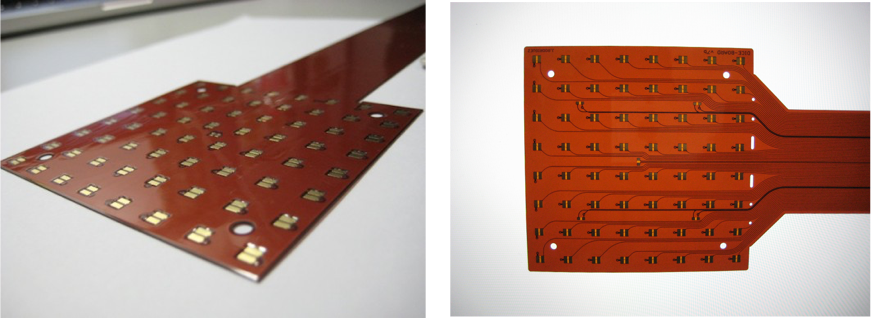
\includegraphics[scale=0.5]{img/KDB2.png}\\
	\caption{\label{fig.KDB} Top and bottom pictures of the Kapton Dice Boards (KDB) developed for the tracking plane of the NEW and NEXT-100 detectors by the NEXT collaboration.}
\end{figure}

In NEW and NEXT-100 the tracking function is provided by a plane of SiPMs operating as light-pixels and located behind the transparent EL grids. They are mounted on flexible radiopure Kapton Dice Boards (KDBs). Each KDB hosts 64 SiPMs (Figure  \ref{fig.KDB}). The NEW  tracking plane is currently being commissioned with 28 KDBs. The NEXT-100 tracking plane will deploy 112 KDBs.  

The dice boards for the LXSC will be built using the technology developed by NEXT. The design is essentially the same, since the SiPMs foreseen for PETALO are of the same type deployed by NEW and NEXT-100 (SENSL C or J series). The main difference is the size of the SIPM (6 mm rather than 1 mm) which however affects very little the design. 

The NEXT KDBs have been developed by the IFIC group during a period of five years. Currently the technology and expertise of the group is very mature and can be reused at a very moderate cost both in terms of money and personnel. 

%PETALO is a liquid-xenon, scintillation based detector with a simpler design and operating conditions  that the NEXT-DEMO, NEW and NEXT-100 detectors. It does not operate at high pressure and does not involve electric fields. Cryogeny at LXe temperatures is rather straight forward and the purification of the gas system much simpler than in the case of NEXT. It will fully benefit from the experience acquired over the last seven years by the IFIC NEXT team. 

\subsubsection*{I3M-UPV group: expertise in the development of ASICS for PET}

The I3M-UPV research team has developed two ASICs for PET applications that
exploit the benefits of analog processing and reduce the number of channels
to acquire thus cutting down the complexity of the following DAQ system. 
The first of them, PESIC\footnote{Herrero-Bosch, V. et al., 
``PESIC: An integrated Front-end for PET
Applications'', Nuclear Science, IEEE Trans. on, vol.55, 2008.} was designed to work mainly with multi-anode
Position Sensitive Photomultiplier Tubes (PSPMT). Its architecture was
designed to improve time behaviour and increase spatial resolution. Its
preamplifying stage introduced two main benefits: digitally programmable gain
adjustment for every photomultiplier output, and isolation from front-end
electronics by means of current buffers. This last feature allows using
different types of photomultipliers such as SiPM and optimises front-end
dead-time, reducing impact position dependent output delay. PESIC used a
resistive charge division network to obtain bi-dimensional information of the
detected event inside a scintillation crystal.  Individual gain control of
the inputs introduced a calibration mechanism close to the detector. This
fine tuning capability improved its overall performance by minimising gain
deviations along the PSPMT sensitive area\footnote{Herrero-Bosch, V et al. ``Position sensitive scintillator based detector
improvements by means of an integrated front-end'', Nuclear Instrument and Methods
A, no.604, 2009.}. However PESIC architecture
was limited to 64 inputs and could not be easily scaled to a higher number
of inputs.

The second ASIC, AMIC\footnote{Herrero-Bosch, V. et al., ``AMIC: An Expandable Front-End for Gamma-Ray
Detectors With Light Distribution Analysis Capabilities'', Nuclear Science,
IEEE Trans. on , vol.58, no.4, 2011.} shared with PESIC a preamplifier stage but carried
out a more complex operation with the inputs. Its unique architecture
allowed carrying out up to 8 parallel calculations with these inputs in the
analog domain. These operations consist of a scaling by an 8 bit precision
digitally configurable coefficient for every input and a sum of the results.
Each one of the fully analog blocks which implemented this basic operation
was named CB (Computational Block). Inside each CB a different set of
coefficients can be programmed so that it can calculate the geometrical
moment of the light distribution obtained from the photodetector. Zero order
moment can be identified with total energy; first order moment is related to
the baricenter of the light distribution and so on. Since the basic
operation is an additive one, the underlying principle of the architecture
can be extended to an arbitrary number of inputs using several AMIC devices
with the right set of coefficients programmed inside. The upper limit of
devices being employed is only limited by the required Signal to Noise Ratio
(SNR). The value of the coefficients may include any calibration needed to
optimise detectors response\footnote{Herrero-Bosch,V.; et al., ``Programmable integrated front-end for
SiPM/PMT PET detectors with continuous scintillating crystal'',
Instrumentation, Journal of , vol.7, Dec. 2012.}. AMIC design was fully developed up to the
industrial level and produced in medium scale for a Spanish medical imaging
company.

\subsubsection*{Expertise of the GIBI230-LaFe group}

The Principal Investigator and the members of the research group form a multidisciplinary team including physicists, nuclear physicians and telecommunications engineers inside the Biomedical Imaging Research Group GIBI230\footnote{http://www.iislafe.es/biomedica-imagen.aspx} . Their experience include:
\begin{enumerate}
\item Development and validation of imaging biomarkers.
\item New techniques and diagnosis based in molecular imaging.
\item Combined analysis of molecular and anatomical information.
\item Definition and implementation of parametric imaging including biological, functional and anatomical information.
\item Safety aspects regarding the use of ionising radiation. 
\end{enumerate}

